\documentclass[11pt, oneside]{article} 
\usepackage{geometry}
\geometry{letterpaper} 
\usepackage{graphicx}
	
\usepackage{amssymb}
\usepackage{amsmath}
\usepackage{parskip}
\usepackage{color}
\usepackage{hyperref}

\graphicspath{{/Users/telliott_admin/Dropbox/Tex/png/}}
% \begin{center} 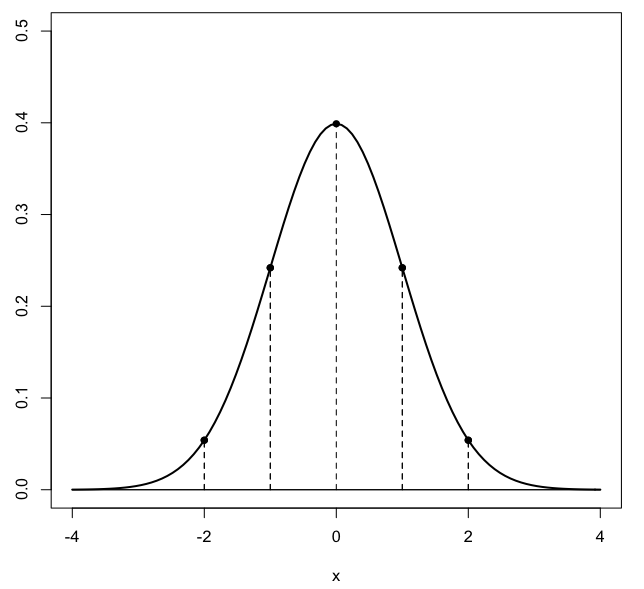
\includegraphics [scale=0.4] {gauss3.png} \end{center}

%break
\title{A famous limit}
\date{}

\begin{document}
\maketitle
\Large

\label{sec:A_famous_limit}

The fundamental result of calculus with respect to trigonometric functions depends on this limit
\[    \lim_{x \rightarrow 0} \ \frac{x}{\sin x}  \]

The limit of the ratio of the angle to its sine as the angle gets very small is equal to $1$.  One way to explore this is to use a plotting application:

\begin{center} 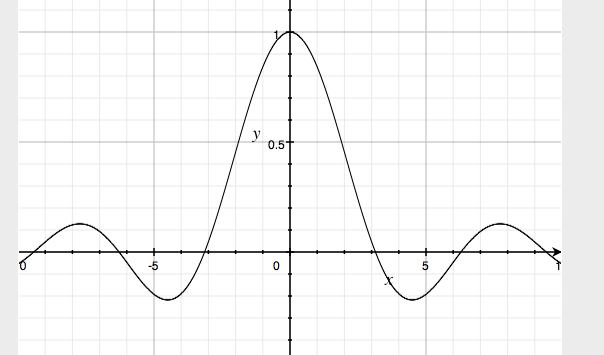
\includegraphics [scale=0.4] {sinx_over_x.png} \end{center}
or a calculator such as that embedded in Python

\begin{verbatim}
>>> for i in range(1,100):
...     f = 1.0/i
...     print i, sin(f)/f
... 
1 0.841470984808
..
97 0.999982286557
98 0.99998264621
99 0.999982995019
>>>
\end{verbatim}

but these are (to be honest) cheating because when they calculate the sine of the angle they use a shortcut based on calculus.

Here is an actual proof that the ratio is equal to $1$.

\begin{center} 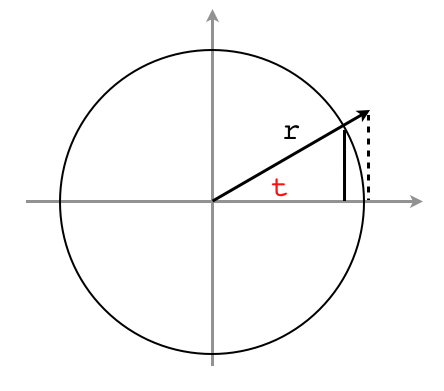
\includegraphics [scale=0.6] {lim_x_over_sinx} \end{center}

Consider the right triangle with radius $r$ (the one that lies entirely inside the circle).  Its base is $r \cos t$ and its height is $r \sin t$, so its area is
\[    A = \frac{1}{2} \cdot r \cos t \cdot r \sin t   \]
\[    = \frac{1}{2} r^2 \sin t \cos t  \]

Consider next the sector of the circle (piece shaped like a slice of pie) containing the same angle, $t$.  Recall that $t$ is the length of the portion of the circumference along this sector (if $t$ is measured in radians).  If the circle is not a unit circle, then multiply by the radius.

The area of the sector could then be approximated as a triangle with base $r \theta$ and height $r$. 

Alternatively, consider that $t$ is some fraction of the total angular measure of the circle, namely $t/2 \pi$, and we multiply by the total area of the circle to get the area of the sector:
\[    A = \frac{t}{2 \pi} \pi r^2 = \frac{1}{2} r^2 t  \]

It's the same answer.

Finally, consider the right triangle containing the dotted line, whose base has length $r$.  Because it is a similar triangle with the first one, its height (that dotted line) is in the same ratio to $r$, the base of the triangle, as $\sin t$ is to $\cos t$.  Thus, its length is $r \tan t$ and so the area of this triangle is
\[   A = \frac{1}{2} \cdot r \cdot r \tan t   \]
\[    =  \frac{1}{2} r^2 \ \frac{\sin t}{\cos t}  \]

Since the first triangle is smaller than the sector, and the sector is smaller than the second triangle, \emph{no matter how small t becomes}:
\[    \frac{1}{2} r^2 \sin t \cos t < \frac{1}{2} r^2 t < \frac{1}{2} r^2 \ \frac{\sin t}{\cos t}  \]

Now cancel $r^2/2$
\[    \sin t \cos t < t < \frac{\sin t}{\cos t}  \]

and divide by $\sin t$
\[    \cos t < \frac{t}{\sin t} < \frac{1}{\cos t}  \]

As $t \rightarrow 0$, both $\cos t$ and $1/\cos t$ approach the same limit, $1$.  Therefore the ratio gets squeezed, and it approaches the same limit as well

Therefore:
\[    \lim_{x \rightarrow 0} \ \frac{x}{\sin x} = 1  \]

\subsection*{Difference quotient for sine}
The limit just obtained will be helpful in finding derivatives of sine and cosine.  Set up the difference quotient for sine:

\[ \frac{\sin (x + h) - \sin x}{(x + h) - x} \]
Using the addition of angles formula
\[ = \frac{\sin x \cos h + \sin h \cos x - \sin x}{h} \]
\[ = \frac{\sin x (\cos h - 1)}{h} + \frac{\sin h \cos x}{h} \]
We want the limit as $h \rightarrow 0$.  The term on the right is
\[ \cos x \ \lim_{h \rightarrow 0} \frac{\sin h}{h} = \cos x \]
The term on the left will be equal to zero
\[ \sin x \  \lim_{h \rightarrow 0} \frac{\cos h - 1}{h} = 0 \]
which means that we have in the end:
\[ \frac{d}{dx} \sin x = \cos x \]
The derivative of the sine is the cosine.

We can massage that extra term as follows:
\[ \frac{\cos h - 1}{h}  \cdot \frac{\cos h + 1}{\cos h + 1} = \frac{\cos^2 h - 1}{h(\cos h + 1)} \]
\[ = \frac{\sin^2 h}{h(\cos h + 1)} \]
\[ = \frac{\sin h}{h} \cdot \frac{\sin h}{\cos h + 1} \]
The limit as $h \rightarrow 0$ of the first factor is equal to $1$ as we saw before, and the second one is $0/2 = 0$, so the whole thing is zero.

\subsection*{Derivative of the cosine}
For the cosine, we \emph{could} set up a difference quotient, but let's do something else just for fun.  Start from
\[ \sin^2 x + \cos^2 x = 1 \]
Using implicit differentiation and the chain rule:
\[ 2 \sin x \ (\frac{d}{dx} \sin x) + 2 \cos x \ (\frac{d}{dx} \cos x) = 0 \]
Plugging in our recent result:
\[ 2 \sin x \cos x + 2 \cos x (\frac{d}{dx} \cos x) = 0 \]
\[ \sin x + (\frac{d}{dx} \cos x) = 0 \]
Rearranging, we get that
\[ \frac{d}{dx} \cos x = - \sin x \]

\subsection*{example}
Here is a problem we can solve using these results.
\begin{center} 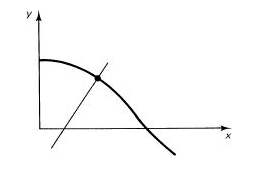
\includegraphics [scale=0.6] {y_cosx.png} \end{center}

The curve is $\cos x$ and the question is, if we form the norm (perpendicular) to the curve, does it ever pass through the origin?

The slope of the tangent is $- \sin x$.  The slope we seek is perpendicular to that, so its product must yield $-1$.  Thus $m = 1/\sin x$.

We use the point slope formula:
\[ \frac{y - y_0}{x - x_0} = \frac{1}{\sin x} \]
At the point $(x_0,y_0) = (0,0)$
\[ \frac{y}{x} = \frac{1}{\sin x} \]
But $y = \cos x$ so
\[ \sin x \cos x = x \]
\[ \frac{1}{2} \sin 2x = x \]
\[ \sin 2x = 2x \]
One solution is $(0,0)$.  Are there any more?  One way to answer this is to go back to the figure we started with where we plot $\sin x/x$:
\begin{center} 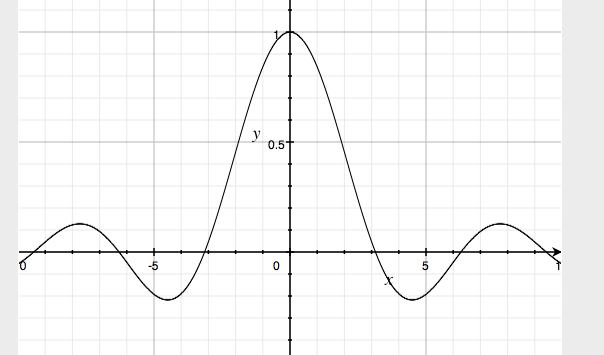
\includegraphics [scale=0.4] {sinx_over_x.png} \end{center}
No.  $\sin x = x$ happens only at $x = 0$  In the figure, $\sin x/ x = 1$ happens only at $x=0$.

For an analytical proof, we observe that the slope of $\sin x$ is equal to $\cos x$ which is equal to $1$ at $x = 0$ and for every $x$ after that
\[ 0 < \cos x < 1, \ \ \ \ 0 < x < \frac{\pi}{2} \]
the slope of $\sin x$ is less than $1$, while the slope of $y = x$ is equal to $1$ everywhere.

The result is that the $x$ rises faster than $\sin x$ everywhere after $x = 0$.

\subsection*{Other trig functions}

We use the quotient rule, described \hyperlink{quotient_rule}{\textbf{here}}.
\[ \frac{u}{v}' = \frac{u'v - uv'}{v^2} \]

Check that we've remembered it correctly:
\[ [ \ \frac{x}{1} \ ] ' = \frac{1 \cdot 1 - x \cdot 0}{1} = 1 \]

The derivative of the tangent is
\[ \ [ \ \frac{\sin x}{\cos x} \ ]' = \frac{\cos x \cdot \cos x - \sin x (- \sin x)}{\cos^2 x} \]
\[ = \frac{1}{\cos^2 x} = \sec^2 x \]
\[ \frac{d}{dx} \ \tan x = \sec^2 x \] 
and the secant:
\[ \ [ \ \frac{1}{\cos x} \ ] ' =  \frac{-(- \sin x)}{\cos^2 x}  \]
\[ = \sec x \tan x \]
\[ \frac{d}{dx} \ \sec x =\sec x \tan x \] 


\end{document}